\section{Experiment 8C: client-level privacy--control frontier}
\label{sec:experiment8c}

\paragraph{Question and threat model.}
Experiment 8C asks how formal client-level privacy affects structured LPV
estimation and downstream control. The protected unit is one vehicle's complete
local identification dataset. Replacement adjacency allows one participating
vehicle to be replaced by any other admissible vehicle. The adversary observes
only the released family aggregate; secure summation is assumed from 8B. The
mechanism does not hide the existence or size of a family, protect against
malicious clients, or include cryptographic overhead. Unlike secure aggregation
alone, differential privacy also limits information in the released aggregate.

\paragraph{One-shot bounded release.}
Every client first fits its local three-ratio model. Let $q_i=\log p_i$. Public
estimator bounds define a center $c$ and half-range vector $s$, giving
$z_i=(q_i-c)\oslash s\in[-1,1]^3$. The contribution is clipped to
$\lVert z_i\rVert_2\le C=\sqrt{3}$. For a family of $n=10$ clients, the
replacement sensitivity of the mean is
\begin{equation}
 \Delta_2=\frac{2C}{n}.
\end{equation}
The released normalized mean is
\begin{equation}
 \widetilde z=\frac1n\sum_{i=1}^n z_i+mathcal N(0,\sigma^2 I_3),
\end{equation}
where $\sigma$ is calibrated with the analytic Gaussian mechanism for the target
$(\epsilon,\delta)$ guarantee \cite{balle2018analytic}. Mapping $\widetilde z$
back into the public parameter box is post-processing. This one-shot release
avoids privacy composition across the iterative queries used in 8B, at the cost
of aggregating local estimates rather than the exact pooled output-error
objective.

\paragraph{Protocol.}
The privacy grid is $\epsilon\in\{0.5,1,2,4,8,\infty\}$ at
$\delta=10^{-5}$. Here $\epsilon=\infty$ is the non-private mean of the same
bounded client contributions. Ten independent privacy draws are evaluated on
each of ten fresh fleets, seeds 71--80, using the 7C single-speed local records.
Every released oracle-Family model is converted to the unchanged scheduled LQI
controller and tested on three nonlinear held-out scenarios. The descriptive
utility gate requires no more than 10\% mean tracking increase relative to the
non-private mean, full amplitude feasibility, and frozen spectral radius below
one. The relative threshold was fixed before execution.

\begin{table}[htbp]
\centering
\caption{Experiment 8C privacy--control frontier. Standard deviation and 95th
percentile use the 100 fleet--privacy-draw units at each finite $\epsilon$;
$\epsilon=\infty$ has ten fleet units.}
\label{tab:experiment8c}
\begin{tabular}{lrrrr}
\toprule
$\epsilon$ & Tracking mean & Tracking SD & Feasible fraction & Max. $\rho$\\
\midrule
0.5 & 1.38393 & 0.80278 & 0.89 & 5.3762\\
1 & 0.96284 & 0.75024 & 0.94 & 3.8755\\
2 & 0.45490 & 0.41700 & 0.99 & 3.4397\\
4 & 0.14038 & 0.09717 & 1.00 & 0.9896\\
8 & 0.06286 & 0.03668 & 1.00 & 0.9806\\
$\infty$ & 0.007432 & 0.000147 & 1.00 & 0.9691\\
\bottomrule
\end{tabular}
\end{table}

\begin{figure}[htbp]
\centering
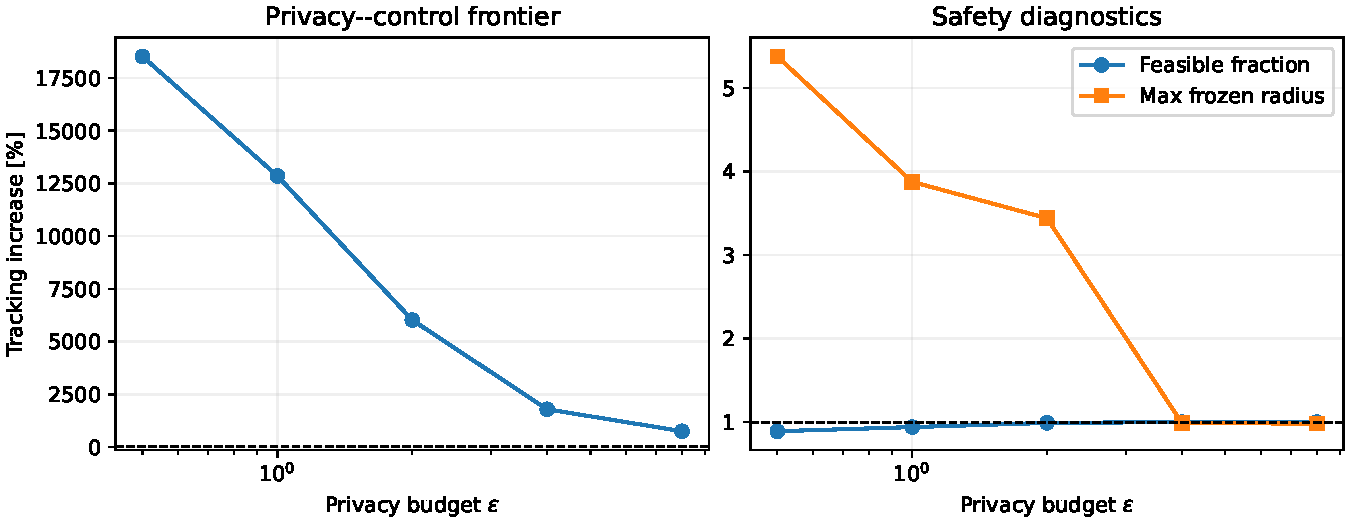
\includegraphics[width=0.86\linewidth]{../results/figures/experiment_8c_private_frontier.pdf}
\caption{Tracking degradation and safety diagnostics versus the client-level
privacy budget. Lower $\epsilon$ gives stronger privacy. The dashed line in the
left panel is the predeclared 10\% utility threshold; the dashed line in the
right panel marks frozen spectral radius one.}
\label{fig:experiment8c}
\end{figure}

\paragraph{Results and interpretation.}
All 300 local fits converge. The study evaluates 1,530 family releases and
45,900 client--scenario closed-loop cases. As \cref{tab:experiment8c,fig:experiment8c}
shows, no finite privacy level satisfies the 10\% gate. At $\epsilon=8$, mean
tracking error is 0.06286 deg/s, 746\% above the unusually small non-private
error of 0.007432 deg/s, although every run remains amplitude-feasible and the
largest frozen radius is 0.9806. At $\epsilon=4$, feasibility also remains
complete, but mean tracking reaches 0.14038 deg/s. For $\epsilon\le2$, at least
one privacy draw has frozen radius above one; feasibility rates are 0.99, 0.94,
and 0.89 for $\epsilon=2,1,0.5$, respectively. The low-$\epsilon$ results must
therefore not be summarized by mean tracking alone.

This failure is structural rather than an optimizer artifact. Replacement-level
sensitivity is $2\sqrt3/10$, so a group of ten provides limited privacy
amplification. Public parameter bounds are broad, and isotropic normalized noise
spends privacy budget on directions with unequal control relevance. Clipping the
released value to the parameter box prevents invalid parameters but cannot
recover the lost vehicle-specific information. Conversely, the large percentage
increases partly reflect an exceptionally accurate non-private baseline; the
absolute errors at $\epsilon=4$ and 8 may still be operationally small, but no
application-derived acceptance limit was available and none is introduced after
seeing the outcomes.

\paragraph{Decision.}
Naive one-shot isotropic client-level DP is not an acceptable final method for
ten-client families under the predeclared relative utility requirement. The
negative result nevertheless gives the FL extension a precise technical target.
The next experiment should test mechanisms that improve privacy utility without
weakening the definition: larger secure-aggregation cohorts, tighter defensible
public bounds, and control-sensitivity-aware anisotropic noise or projection.
Any such mechanism must retain the same $(\epsilon,\delta)$ adjacency statement
and be compared on fresh privacy draws. Record-level privacy or a larger
$\epsilon$ must not be substituted silently.

\paragraph{Reproducibility.}
The protocol is \path{code/config/experiment_8c.json}; the runner is
\path{code/experiments/experiment_8c_private_frontier.py}; analytic calibration
and transformations are in \path{code/src/federated_lpv/privacy.py}. Per-seed
compressed files retain local fits, every privacy draw, Gaussian scale, noise
norm, released parameter, and client-level closed-loop metrics.
